\label{apprentissage_auto}

\subsection{Principes fondamentaux}

\label{apprentissage_automatique_principes}

L'apprentissage automatique supervisé (ou apprentissage artificiel supervisé) définit un certain nombre de méthodes permettant d'effectuer des prédictions pour résoudre des problèmes. Ces méthodes sont appelées « modèles », et correspondent aux différents algorithmes utilisés pour extraire la connaissance d'un ensemble d'exemples, puis pour effectuer des prédictions sur des exemples inconnus. Avant d'effectuer des prédictions, les modèles doivent en effet d'abord suivre une phase d'apprentissage (ou d'entraînement), pendant laquelle leurs paramètres internes sont ajustés pour effectuer la bonne prédiction en fonction des données en entrée. Dans le cas qui nous intéresse, ces prédictions peuvent être une valeur ou un ensemble de valeurs, on parle alors d'une tâche de régression. Lors de la phase d'entraînement, la distance entre la prédiction d'un modèle et la valeur cible qui était attendue pour chaque exemple lui est donnée. Ce mécanisme lui permet d'ajuster itérativement ses paramètres internes, et est à l'origine de la qualification d'apprentissage supervisé.


\subsubsection{Séparation des jeux de données}

\label{apprentissage_automatique_separation_jeux}

\par Lorsque l'on élabore un modèle prédictif, il n'est pas souhaitable d'évaluer ses performances sur les données qui ont servi à son entraînement. Cela induirait en effet un biais important, du fait qu'il est possible qu'il devienne très performant pour prédire les données qu'il connaît, mais qu'il ne soit pas capable de généraliser ses connaissances à des données qui lui sont inconnues (\ref{sur_ajustement}). C'est pour cette raison que l'on sépare généralement les données en deux jeux disjoints : un jeu d'entraînement sur lequel le modèle effectue son apprentissage, et un jeu de test (ou de validation) sur lequel ses performances sont évaluées.

\subsubsection{Validation croisée}

\label{apprentissage_automatique_validation_croisée}

\par Pour évaluer les performances d'un modèle, il est intéressant d'évaluer ses performances lorsqu'il s'entraîne sur des jeux de données différents, la qualité des prédictions d'un modèle pouvant varier d'un entraînement à un autre. Une technique répandue pour évaluer la variance des performances d'un modèle est celle de la validation croisée à $n$ entraînements. Elle consiste à séparer le jeu d'entraînement en $n$ sous-ensembles disjoints nommés plis, puis à effectuer $n$ entraînements sur toutes les combinaisons telles que $n-1$ plis constituent le jeu d'apprentissage, et le dernier pli forme le jeu de test. On peut alors étudier la performance moyenne du modèle, ainsi que la dispersion de la qualité de ses prédictions.


\subsubsection{Recherche des paramètres optimaux}

\label{apprentissage_automatique_quadri}
\par En plus des paramètres internes, les modèles présentent également un certain nombre de paramètres permettant de régler leurs représentations internes ou leurs phases d'apprentissage. Ces paramètres sont parfois appelés hyper-paramètres. Lorsque l'on élabore un modèle, il faut alors également préciser leurs valeurs.\\
\par Pour déterminer un ensemble d'hyper-paramètres optimal ou du moins efficace, la technique la plus répandue est celle de la recherche par quadrillage, éventuellement avec validation croisée. Elle consiste à définir une grille de paramètres, soit un tableau à deux dimensions, contenant pour chaque paramètre (ligne) un ensemble de valeurs (colonnes). Pour chaque combinaison des valeurs, un modèle est entraîné, puis la performance relative des différents modèles est évaluée à la fin de la recherche. Dans le cas d'une recherche par quadrillage avec validation croisée à $n$ entraînements, chaque combinaison de paramètres est testée $n$ fois, ce qui permet en outre de tester la variance des performances de chaque combinaison.

\subsubsection{Prévention du sur-ajustement}
\label{sur_ajustement}

\par Lorsque les données représentent des connaissances trop simples pour un modèle, ou réciproquement que les paramètres internes d'un modèle permettent de représenter des connaissances plus complexes que celles des données, la phase d'entraînement du modèle risque de mener à sur-ajustement (ou sur-apprentissage) des données. Cela signifie que le modèle effectuera de bonnes prédictions sur les données d'entraînement, mais que les connaissances extraites par le modèle se généraliseront mal à de nouvelles données, du fait de leur trop grande spécificité aux données d'apprentissage.\\
\par Pour parer à cela, les différents modèles proposent des techniques de régularisation qui leur sont propres, et qui vont permettre de limiter leur liberté à ajuster de trop près les données d'entraînement.


\subsection{Entraînement de réseaux de neurones artificiels}

\label{apprentissage_automatique_nn}

\subsubsection{Principe}
\par Les réseaux de neurones artificiels sont des modèles prédictifs qui possèdent l'avantage d'être en général plus efficaces que les autres types de modèles sur des jeux de données de grande taille. Ils ont également montré de très bonnes performances comparativement aux autres types de modèles sur des problèmes de traitement de signaux et de traitement d'images.\\

\par L'objectif de ces réseaux de neurones est d'approximer la fonction qui à chaque exemple donné en entrée associe l'ensemble de valeurs attendu en sortie. Ils sont pour cela composés d'un ensemble de neurones artificiels partageant des connexions. L'information circule de l'entrée à la sortie du modèle, en étant transformée successivement par les différents neurones, jusqu'à idéalement prendre la valeur attendue en sortie.\\

\par Chaque neurone est défini par l'ensemble des neurones dont la sortie constitue son entrée, un ensemble de poids, un seuil, une fonction d'activation, ainsi que par l'ensemble des neurones dont l'entrée contient sa sortie. Nous formalisons le fonctionnement d'un neurone de la façon suivante.\\
Soit $n$ la taille de l'entrée d'un neurone, $x_i$ sa $i$\up{ème} entrée, $w_i$ le poids associé à sa $i$\up{ème} entrée ($i \in \{1, ..., n\}$) , $\Theta$ son seuil et $\varphi$ sa fonction d'activation. La somme de $\sum\limits_{i=1}^n w_ix_i$ et de $\Theta$ est transmise à la fonction d'activation, dont la sortie $O$ constitue la sortie du neurone. La valeur $O$ est alors propagée aux neurones suivants.
Ce mécanisme est schématisé dans la figure \ref{neurone}.\\

\begin{figure}
	\centering
	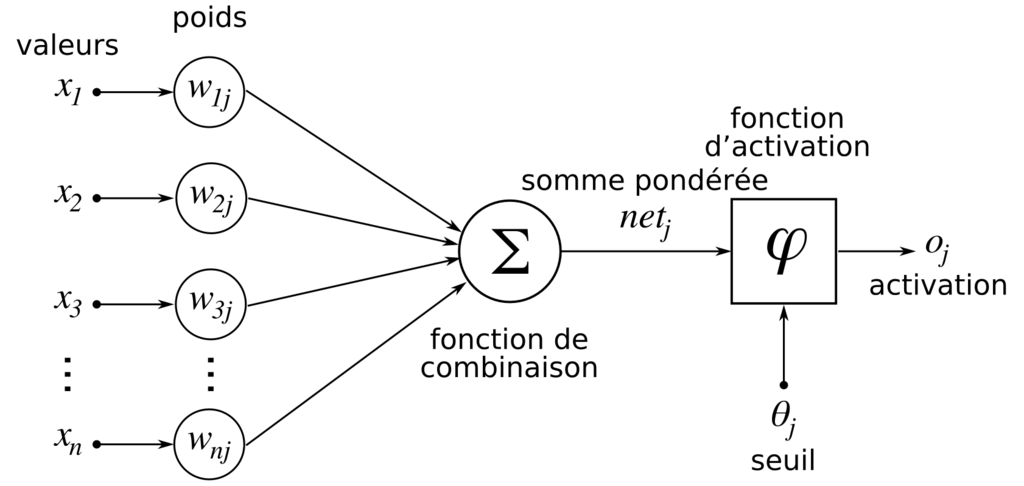
\includegraphics[scale=0.3]{images/neurone.png}
	\caption{Schématisation du fonctionnement d'un neurone artificiel (Wikimedia, Chrislb)}
	\label{neurone}
\end{figure}

\par La phase d'entraînement d'un réseau de neurones est un problème d'optimisation visant à trouver un ensemble de paramètres $w_i$ et $\Theta$ pour chaque neurone du réseau, qui minimise une fonction de coût évaluant la qualité des prédictions.

\subsubsection{Bibliothèque logicielles}

\label{apprentissage_automatique_bibli_log}

\par La totalité du code développé lors de ce projet l'a été dans le langage Python.\\

\par Pour l'implémentation des réseaux de neurones, nous utilisons la bibliothèque Tensorflow\cite{tf} développée par Google, par l'intermédiaire de la surcouche TFLearn\footnote{http://tflearn.org}, qui offre une interface simplifiée pour créer des réseaux de neurones aux architectures communes.\\

\par Nous utilisons de plus la bibliothèque Scikit-Learn\cite{sklearn}, qui permet d'automatiser un certain nombre de tâches liées à l'apprentissage automatique.\\

\par Nous utilisons en outre l'interface web Tensorboard, incluse dans Tensorflow, qui permet de visualiser l'évolution des différentes métriques évaluant la qualité des modèles au cours de l'entraînement.\\

\par Enfin, nous utilisons les notebooks Jupyter\cite{jupyter}, qui permettent d'expérimenter simplement des algorithmes de génération de données ou d'entraînement de modèles, et de présenter les résultats de manière claire.

\subsubsection{Hyper-paramètres}

\label{apprentissage_automatique_parametres_nn}

\par Les modèles crées par l'intermédiaire de TFLearn présentent un certain nombre d'hyper-paramètres (\ref{apprentissage_automatique_principes}), qui permettent de régler finement les modèles que l'on entraîne. Nous listons ci-dessous ces différents paramètres et leurs rôles.

\paragraph{Optimiseur : } Définit la méthode d'optimisation des poids utilisée à chaque étape de l'entraînement. Nous utilisons pour tous les modèles l'optimiseur Adam\cite{adam}, réputé pour être efficace et éviter les minimums locaux de la fonction de coût.

\paragraph{Taux d'apprentissage (\emph{learning rate}) : } Définit la vitesse maximale à laquelle l'optimiseur va modifier les solutions pendant l'optimisation des poids lors de l'entraînement des modèles. Si la valeur est trop faible, l'entraînement mettra trop de temps à converger vers de bonnes solutions. Si elle est trop élevée, le modèle risque d'être bloqué dans des minimums locaux de la fonction de coût.

\paragraph{Epsilon : } Paramètre de l'optimiseur Adam.

\paragraph{Taille de lot (\emph{batch size)} :} L'apprentissage des réseaux de neurones artificiels ne s'effectue pas exemple par exemple mais lot d'exemples par lot d'exemples. Ce paramètre définit la taille de ces lots.

\paragraph{Époques (\emph{epochs})} : Définit le nombre d'époques d'entraînement. Cela correspond au nombre de fois que le réseau de neurones va apprendre sur toutes les données du jeu d'entraînement.

\paragraph{Initialisation des poids : } Les poids du réseau de neurones doivent être initialisés à des valeurs non nulles pour que l'information puisse se propager. Ce paramètre correspond à l'écart-type de la variable aléatoire gaussienne utilisée pour initialiser les poids.

\paragraph{Fonctions d'activation : } Définit les fonctions d'activation utilisées par les neurones artificiels. On différencie la fonction utilisée par les neurones des couches internes de la fonction utilisée par les neurones de la couche de sortie.

\paragraph{Dégradation des poids (\emph{weight decay}) : } Il s'agit d'un paramètre de régularisation ajoutant un terme à la fonction de coût, qui va forcer les poids à ne pas prendre de valeurs trop élevées. La présence de poids possédant des valeurs élevées est en effet un facteur de sur-ajustement\cite{weight_decay}.

\paragraph{Taux d'abandon (\emph{dropout}) : } Technique de régularisation permettant d'éviter le sur-ajustement. À chaque époque d'entraînement, certains neurones sont désactivés aléatoirement afin de pousser le modèle à être résilient et à éviter qu'une co-dépendance forte entre certains neurones s'installe. Ce paramètre permet en réalité de définir la proportion de neurones qui resteront activés à chaque époque.



